

%                I feel like we need some chart here to show how precision scales intuitively for folks (i.e, what’s in the experiments could come up here).

%                Hyperbolics produce low distortion and even low MAP for short bushy… also back this up with numbers from your experiments!
%                Say that the scale is critically important here. Explain that you can simply add in a learnable scale parameter. Mention a micro experiment where it has an impact, and then comment if you think it’s important more broadly.
%            Now you can devote as much as you want to the proof. 
%                You could just give the intuition of each (the precision and the lower bound).
%                I think it’s fine to say this is the key element of the proof.  
%        Embedding trees. Figure 4 is very good. 
%            You should push credit to Abraham earlier (when you mention Steiner nodes). Our contribution is applying them to these embeddings, we build on their iddeas.
%             Line 284. Probably make the is an example environment. Make sure it’s clear the reader needs to transition.
%            Make sure this section is a little more sandwich method (you don’t tell them up front—need more signposting)

We first focus on hyperbolic tree embeddings---a natural approach
considering the tree-like behavior of hyperbolic space.  We
review the embedding of \citet{sarkar} to higher dimensions. We then
provide novel analysis about the precision of the embeddings that
reveals fundamental limits of hyperbolic embeddings. In particular, we
characterize the bits of precision needed for hyperbolic
representations. We then extend the construction to $r$ dimensions,
and we propose to use Steiner nodes to better embed general graphs as
trees building on a condition from \citet{Abraham}.

\paragraph*{Embedding trees} The nature of hyperbolic space lends itself towards excellent tree embeddings. In fact, it is possible to embed trees into the Poincar\'{e} disk $\mathbb{H}_2$ with arbitrarily low distortion \cite{sarkar}. Remarkably, trees cannot be embedded into Euclidean space with arbitrarily low distortion for \emph{any} number of dimensions. These notions motivate the following two-step process for embedding hierarchies into hyperbolic space.
\begin{enumerate}
  \setlength\itemsep{0em}
\item Embed the graph $G=(V,E)$ into a tree $T$,
\item Embed $T$ into the Poincar\'{e} ball $\mathbb{H}_d$.
\end{enumerate}

We refer to this process as the \emph{combinatorial construction}. Note that we are not required to minimize a loss function. We begin by describing the second stage, where we extend an elegant construction from \citet{sarkar}. 

\subsection{Sarkar's Construction}
Algorithm~\ref{alg:sarkar} implements a simple embedding of trees into $\mathbb{H}_2$. The algorithm takes as input a scaling factor $\tau$ a node $a$ (of degree $\operatorname{deg}(a)$) from the tree with parent node $b$. Suppose $a$ and $b$ have already been embedded into $\mathbb{H}_2$ and have corresponding embedded vectors $f(a)$ and $f(b)$. The algorithm places the children $c_1, c_2, \ldots, c_{\operatorname{deg}(a)-1}$ into $\mathbb{H}_2$ through a two-step process. 

First, $f(a)$ and $f(b)$ are reflected across a geodesic (using circle inversion) so
that $f(a)$ is mapped onto the origin $0$ and $f(b)$ is mapped onto some point $z$.
% We compute the angle of $Z'$.
Next, we place the children nodes to vectors $y_1, \ldots, y_{d-1}$ equally spaced around a circle with radius $\frac{e^\tau-1}{e^\tau+1}$ (which is a circle of radius $\tau$ in the hyperbolic metric), and maximally separated from the reflected parent node embedding $z$. Lastly, we reflect all of the points back across the geodesic. 
Note that the isometric properties of reflections imply that all children are now at hyperbolic distance exactly $\tau$ from $f(a)$.

\begin{algorithm}[t]
\begin{algorithmic}[1]
\STATE \textbf{Input:} Node $a$ with parent $b$, children to place $c_1, c_2, \ldots, c_{\operatorname{deg}(a)-1}$, partial embedding $f$ containing an embedding for $a$ and $b$, scaling factor $\tau$
\STATE $(0, z) \leftarrow \operatorname{reflect}_{f(a) \rightarrow 0}(f(a),f(b))$ %\COMMENT{circle inversion}
\STATE $\theta \leftarrow \operatorname{arg}(z)$ \hspace{2em} \COMMENT{angle of $z$ from x-axis in the plane}
\FOR{$i \in \{1, \ldots, \operatorname{deg}(a)-1 \}$}
\STATE $y_i \leftarrow \left(\frac{e^\tau-1}{e^\tau+1} \cdot \cos\left(\theta + \frac{2\pi i}{\operatorname{deg}(a)} \right) , \frac{e^\tau-1}{e^\tau+1} \cdot \sin\left(\theta+\frac{2\pi i}{\operatorname{deg}(a)}\right) \right)$ % \label{alg:sarkar:step:circle}
\ENDFOR
\STATE $(f(a), f(b), f(c_1),\ldots,f(c_{\operatorname{deg}(a)-1})) \leftarrow \operatorname{reflect}_{0 \rightarrow f(a)}(0, z, y_1, \ldots, y_{\operatorname{deg}(x)-1})$
\STATE \textbf{Output:} Embedded $\mathbb{H}_2$ vectors $f(c_1), f(c_2), \ldots, f(c_{\operatorname{deg}(a)-1})$
\end{algorithmic}
\caption{Sarkar's Construction}
\label{alg:sarkar}
\end{algorithm}

To embed the entire tree, we place the root at the origin $O$ and its children in a circle around it (as in Step~5 of Algorithm~\ref{alg:sarkar}), then recursively place their children until all nodes have been placed. Notice this construction runs in linear time.

\subsection{Analyzing Sarkar's Construction}
\label{sec:sarkar}
The \emph{Voronoi cell} around a node $a \in T$ consists of points $x \in \mathbb{H}_2$ such that $d_H(f(a),x) \leq d_H(f(b),x)$ for all $b \in T$ distinct from $a$. That is, the cell around $a$ includes all points closer to $f(a)$ than to any other embedded node of the tree. Sarkar's construction produces Delauney embeddings: embeddings where the Voronoi cells for points $a$ and $b$ touch only if $a$ and $b$ are neighbors in $T$. Thus this embedding will preserve neighborhoods.

A key technical idea exploited by \citet{sarkar} is to scale all the
edges by a factor $\tau$ before embedding. We can then recover the original distances
by dividing by $\tau$. This transformation exploits the fact that
hyperbolic space is not {\em scale invariant}.
Sarkar's construction always captures neighbors perfectly, but Figure~\ref{fig:geod} implies that increasing the scale preserves the distances between farther nodes better.
Indeed, if one sets
$\tau
= \frac{1+\varepsilon}{\varepsilon}\left(2\log \frac{\operatorname{deg}_{\max}}{\pi
/2}\right)$, then the worst-case distortion $D$ of the resulting embedding is no more than
$1+\varepsilon$. For trees, Sarkar's construction has arbitrarily high
fidelity. However, this comes at a cost: the scaling $\tau$ affects
the bits of precision required. In fact, we will show that the
precision scales logarithmically with the degree of the tree---but linearly with the maximum path length. We use
this to better understand the situations in which hyperbolic
embeddings obtain high quality.

%Algorithm~\ref{alg:sarkar} produces edges scaled by $\nu$. That is, a unit distance has been scaled to $\nu$, and we can recover the original distances by dividing by $\nu$. Choosing $\nu$ correctly allows us to bound the distortion $d_{wc}$ of the embedding to $1+\varepsilon$ for any $\varepsilon > 0$.


%We call this Sarkar's condition.

%We build on the $\mathbb{H}_2$ construction from \citet{sarkar}. This approach produces Delauney embeddings, i.e., embeddings $f$ where the Voronoi cells for points $f(x),f(y)$ \footnote{The \emph{Voronoi cell} around $f(x)$ consists of points $\alpha \in \mathbb{H}_2$ such that $d_H(f(x),\alpha) \leq d_H(f(y),\alpha)$ for all $y \in T$ distinct from $x$. That is, the cell around $f(x)$ includes all points closer to $f(x)$ than any other embedded vertex of the tree.} touch only if $x,y$ are neighbors in $T$. The basic idea is to embed the children of $x$ so that each child is placed inside a disjoint cone emanating from $x$. Moreover, the cones rooted at child $y$ lie inside the cone rooted at $x$ containing $y$, so that Voronoi cells around nodes in different subtrees cannot touch. Full details on this approach are found in \citet{sarkar}.

How many bits of precision do we need to represent points in
$\mathbb{H}_2$? If $x \in \mathbb{H}_2$, then $\|x \| < 1$, so we need
sufficiently many bits so that $1 - \|x\|$ will not be rounded to zero. This requires
roughly $-\log (1-\|x\|) = \log \frac{1}{1-\|x\|}$ bits.  Say we are
embedding two points $x,y$ at distance $d$. As described in the
background, there is an isometric reflection that takes a pair of points $(x,y)$
in $\mathbb{H}_2$ to $(0,z)$ while preserving their distance, so
without loss of generality we have that
\[ d = d_H(x, y) = d_H(0,z) = \acosh \left(1+2\frac{\|z\|^2}{1-\|z\|^2} \right). \]
Rearranging the terms, we have \[\frac{\cosh(d)+1}{2} = \frac{1}{1-\|z\|^2} \ge \frac{1/2}{1-\|z\|}.\] Thus, the number of bits we want so that $1 - \|z\|$ will not be rounded to zero is $\log ( \cosh(d)+1)$. Since $\cosh(d) = (\exp(d)+\exp(-d))/2$, this is roughly $d$ bits.
That is, in hyperbolic space, we need about $d$ bits to express distances of $d$ (rather than $\log d$ as we would in Euclidean space).%
\footnote{Although it is particularly easy to bound precision in the Poincar{\'e} model, this fact holds generally for hyperbolic space independent of model. See Appendix~\ref{app:CombinatorialProofs} for a general lower bound argument.}
This result will be of use below.

Now we consider the largest distance in the embeddings produced by Algorithm~\ref{alg:sarkar}. If the longest path in the tree is $\ell$, and each edge has length $\tau = \frac{1}{\varepsilon}\left(2\log \frac{\operatorname{deg}_{\text{max}}}{\pi /2}\right)$, the largest distance is $O(\frac{\ell}{\varepsilon}\log \operatorname{deg}_{\text{max}})$, and we require this number of bits for the representation.

We interpret this expression. Note that $\operatorname{deg}_{\max}$ is inside the $\log$ term, so that a bushy tree is not penalized much in precision. On the other hand, the longest path length $\ell$ is not, so that hyperbolic embeddings struggle with long paths. 
Moreover, by selecting an explicit graph, we derive a matching lower
bound, concluding that to achieve a distortion $\varepsilon$, any
construction requires $\Omega\left(\frac{\ell}{\varepsilon} \log (\text{deg}_{\max}) \right)$
bits, which matches the upper bound of the combinatorial
construction. The argument follows from selecting a graph consisting
of $m(\text{deg}_{\max}+1)$ nodes in a tree with a single root and $\text{deg}_{\max}$ chains each of length $m$. The
proof of this result is described in Appendix~\ref{app:CombinatorialProofs}.

%% \begin{figure}
%% \centering
%% 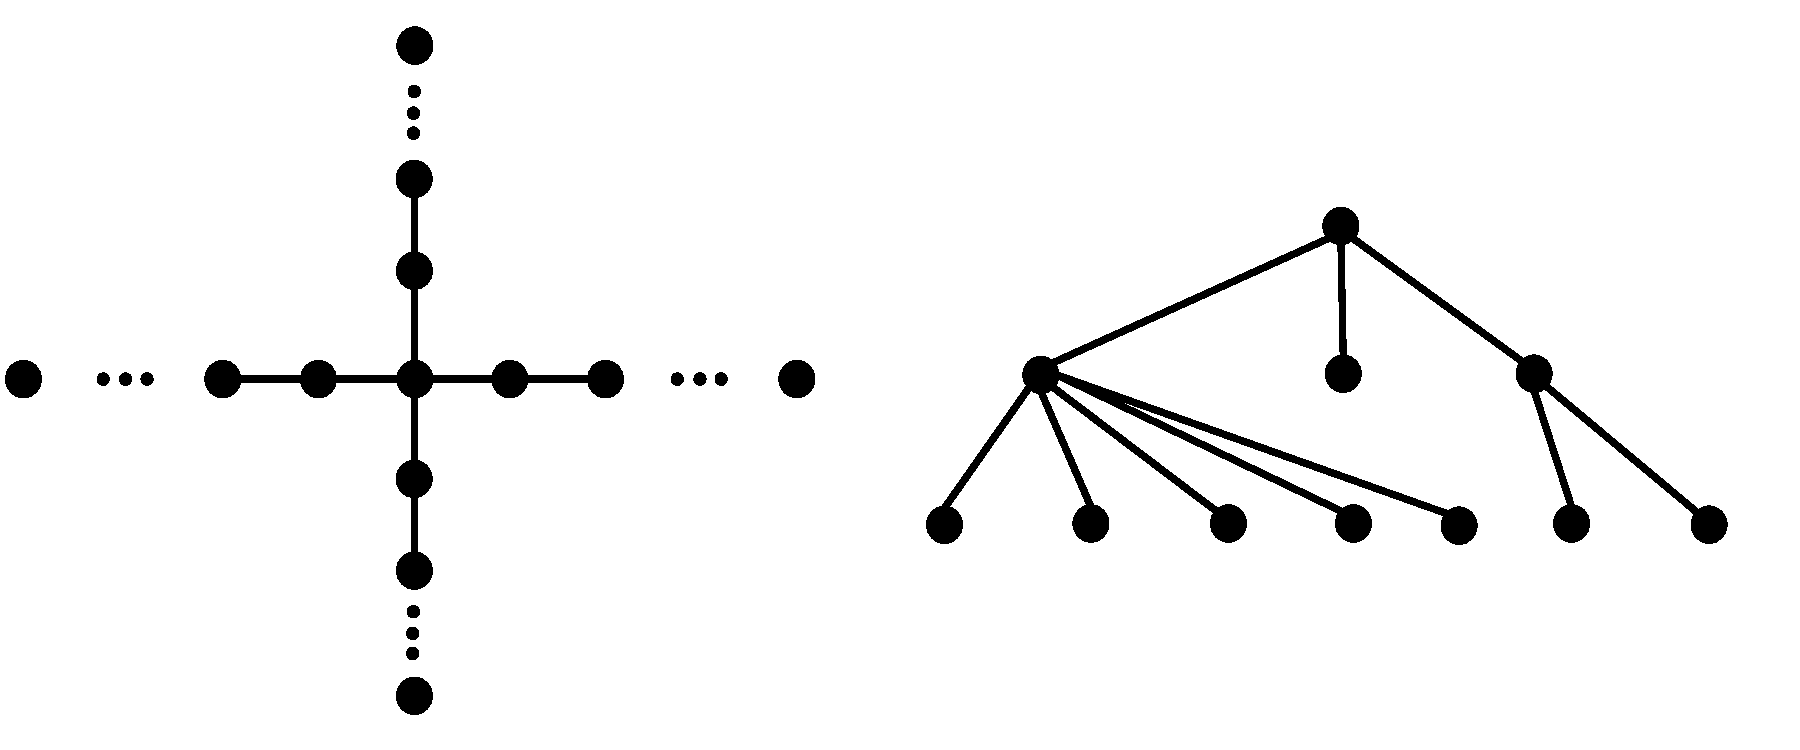
\includegraphics[width=0.50\textwidth]{figures/chain2.pdf}
%% \caption{Graphs with long chains are difficult for hyperbolic embeddings (left) while short bushy trees are easy (right).}
%% \label{fig:chains}
%% \end{figure}

%Our implementation of the construction follows \cite{Sarkar} closely, with simple modifications required by the fact that in \cite{Sarkar}, the construction is performed in (abstract) hyperbolic space, while we work with the Poincar\'{e} models. 

\subsection{Improving the Construction}



%\begin{table}[tb]
%\centering
%\begin{tabular}{|l||c|c|c|c|c|}
%\hline 
%Dataset & Nodes & $d_{\max}$ &  $r=2$ & $r=3$ & $r=5$ \\    \hline    \hline
%Bal. Tree     & 40    &4  & 25 & 13  & 13 \\ \hline
%Phy. Tree & 344  &16 & 425 & 142 & 107\\ \hline
%\end{tabular}
%\caption{Precision upper bound required for combinatorial construction at $\varepsilon=1.0$ tolerance for two trees described in Section~\ref{sec:experiments}.}
%\label{table:bitcost}
%\end{table}

Our next contribution is a generalization of the construction from the disk $\mathbb{H}_2$ to the ball $\mathbb{H}_r$. Our construction follows the same line as Algorithm~\ref{alg:sarkar}, but since we have $r$ dimensions, the step where we place children spaced out on a circle around their parent now uses a hypersphere.

Spacing out points on the hypersphere is a classic problem known as \emph{spherical coding} \cite{Spheres}. As we shall see, the number of children that we can place for a particular angle grows with the dimension. Since the required scaling factor $\tau$ gets larger as the angle decreases, we can reduce $\tau$ for a particular embedding by increasing the dimension. Note that increasing the dimension helps with bushy trees (large $\operatorname{deg}_{\max}$), but has limited effect on tall trees with small $\operatorname{deg}_{\max}$. We show

%there are $r-1$ angles $\theta_1, \ldots, \theta_{r-1}$. We divide the angles into $k$ parts, allowing us to place $\Theta(k^{r-1})$ children around any node for $k\geq 2$. Since we need $k^{r-1} \geq \operatorname{deg}_{\max}$, we can ultimately reduce the precision linearly in $r$ for $r$ up to $\leq (\log \operatorname{deg}_{\max})+1$. 


\begin{proposition} The generalized $\mathbb{H}_r$ combinatorial construction has distortion at most $1+\varepsilon$ and requires at most $O(\frac{1}{\varepsilon}\frac{\ell}{r} \log \operatorname{deg}_{\max})$ bits to represent a node component for $r \leq (\log \operatorname{deg}_{\max})+1$, and $O(\frac{1 }{\varepsilon}\ell)$ bits for $r > (\log \operatorname{deg}_{\max})+1$. 
\end{proposition}

The algorithm for the generalized $\mathbb{H}_r$ combinatorial construction replaces Step~5 in Algorithm~\ref{alg:sarkar} with a node placement step based on ideas from coding theory. The children are placed at the vertices of a hypercube inscribed into the unit hypersphere (and afterwards scaled by $\tau$). Each component of a hypercube vertex has the form $\frac{\pm 1}{\sqrt{r}}$. We index these points using binary sequences ${a} \in \{0,1\}^r$ in the following way:

\[{x}_{ a} = \left( \frac{(-1)^{a_1}}{\sqrt{r}}, \frac{(-1)^{a_2}}{\sqrt{r}} , \ldots, \frac{(-1)^{a_r}}{\sqrt{r}} \right).\]

We can space out the children by controlling the distances between the children. This is done in turn by selecting a set of binary sequences with a prescribed minimum Hamming distance---a binary error-correcting code---and placing the children at the resulting hypercube vertices. We provide more details on this technique and our choice of code in the appendix.
%\begin{proof}
%Our argument connects the required edge lengths for Sarkar's condition to be met, and the number of children we can place around a node $k^{r-1}$. We require $k^{r-1} \geq d_{\max}$.

%First, we can simplify our analysis by isometrically reflecting hyperbolic space so that the parent $x$ is the origin $0$. Let this isometry take $y$ to $p$. Then, using the hyperbolic distance formula, \begin{align*} d_H&(x,y) = d_{H}(0,q) = \\ &\mathsf{acosh}\left(1 + \frac{\cos^2 \theta/2}{1 - \cos^2 \theta/2}\right) = 
 % \mathsf{acosh}\left(1 + \cot \frac{\theta}{2}\right).\end{align*}
%Now we estimate $\exp\{ d_H(x,y) \} - 1 =  \cot \frac{\theta}{2}$ yielding $\tan \frac{\theta}{2} \leq \exp\{ - d_H(x,y) \}.$

%We place rays spaced at intervals of $\pi/k$ emanating from a point in each dimension. The cones are placed aligned with these rays. The resulting lattice can thus hold $k^{r-1}$ cones. In order to place all the children of each node, we must have $k^{r-1} \geq d_{\max}$. 
%Then, the edge lengths satisfy
%\begin{align*}
%-\log &\tan \frac{\pi}{2k} = - \log \tan \frac{\pi d_{\max}^{-1/r}}{2} \approx - \log \frac{\pi d_{\max}^{-1/r}}{2} \\
%&=  \frac{1}{r} \log d_{\max} - \log \frac{\pi}{2}.
%    \end{align*}
%We only need to meet Sarkar's condition, which offers $1+\varepsilon$ distortion if each length is scaled by the former quantity times $\frac{1+\varepsilon}{\varepsilon}$. Thus we meet our distortion bound. Next, recall that for a node component, the representation requires no more bits than the maximum path length $\ell$ times the edge length for our tree; this quantity is given by 
%\begin{equation}
%O\left(\frac{1 +  \varepsilon}{\varepsilon}\frac{\ell}{r} \log d_{\max} \right),
%\label{eq:prec}
%\end{equation}
%as desired.
%\end{proof}. 

%Observe that the precision has now been decreased by a factor of $r$, the dimension.

%To gain intuition about the precision-dimension tradeoff,
%Table~\ref{table:bitcost} shows the precision bound as the embedding dimension changes for two trees.
% The key takeaways of our analysis are:
% \begin{itemize}
%   \setlength\itemsep{0em}

% \item
% There is a fundamental tension between precision and quality in
% hyperbolic embeddings.

% \item Hyperbolic embeddings have an exponential advantage in space compared to Euclidean embeddings for short, bushy hierarchies, but will have less of an advantage
% for graphs that contain long paths.

% \item Choosing an appropriate scaling factor $\tau$ is critical for quality.
% Later, we will propose to learn this scale factor automatically for computing embeddings in PyTorch.
% \end{itemize}




\subsection{Embedding into Trees}
%Since embedding trees into the Poincar\'{e} can be performed with distortion as low as we desire, it remains to consider the distortion in the first stage. 
\begin{figure}
\centering
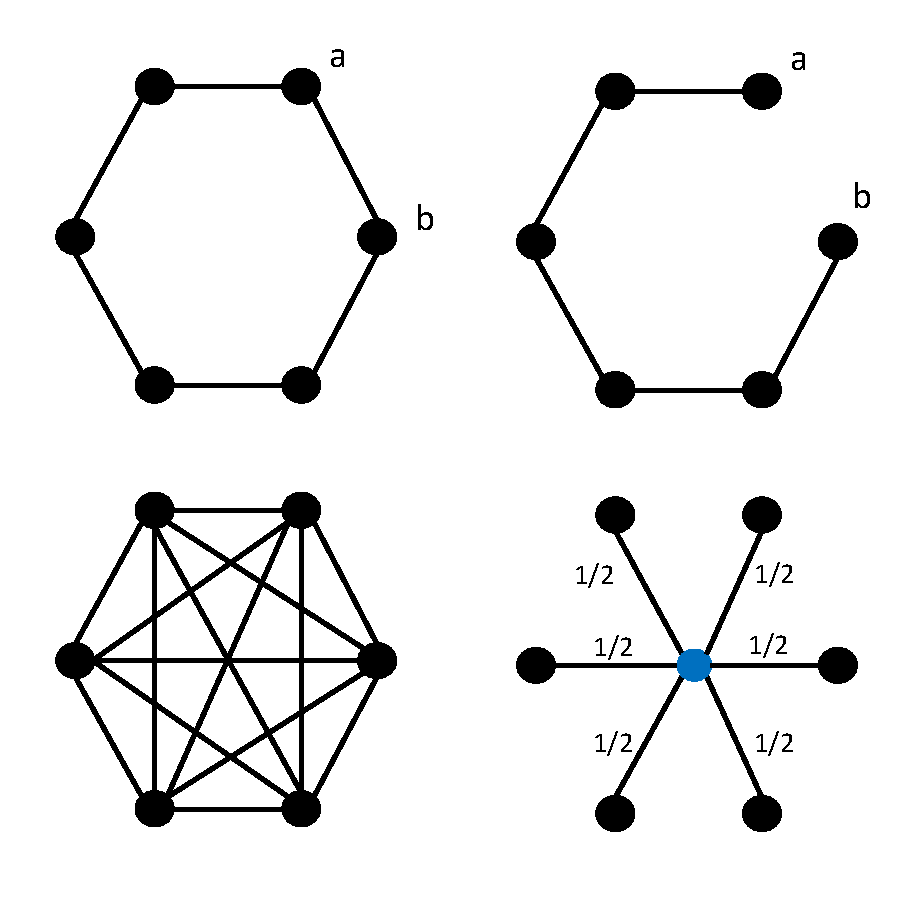
\includegraphics[width=0.3\textwidth]{figures/steiner.pdf}
\caption{Top. Cycles are a challenge for tree embeddings: $d_G(a,b)$ goes from $1$ to $5$. Bottom. Steiner nodes can help: adding a node (blue) and weighting edges maintains the pairwise distances.}
\label{fig:steiner}
\end{figure}
We revisit the first step of the construction: embedding graphs into
trees. There are fundamental limits to how well graphs can be embedded
into trees; in general, breaking long cycles inevitably adds
distortion, as shown in Figure~\ref{fig:steiner}. We are inspired by a
measure of this limit, the \emph{$\delta$-4 points condition} introduced
in \citet{Abraham}. A graph on $n$ nodes that satisfies the $\delta$-4
points condition has distortion at most $(1+\delta)^{c_1 \log n}$ for
some constant $c_1$. This result enables our end-to-end embedding to
achieve a distortion of at most \[D(f) \leq (1+\delta)^{c_1 \log n}(1
+ \varepsilon).\]

The result in \citet{Abraham} builds a tree with \emph{Steiner} nodes. These additional nodes can help control the distances in the resulting tree.
\begin{example} \label{ex:steiner}
Embed a complete graph on $\{1,2,\ldots, n\}$ into a tree. The tree will have a central node, say 1, w.l.o.g., connected to every other node; the shortest paths between pairs of nodes in $\{2,\ldots,n\}$ go from distance 1 in the graph to distance 2 in the tree. However, we can introduce a Steiner node $n+1$ and connect it to all of the nodes, with edge weights of $\frac{1}{2}$. This is shown in Figure~\ref{fig:steiner}. The distance between any pair of nodes in $\{1,\ldots,n\}$ remains 1.\end{example}

Note that introducing Steiner nodes can produce a weighted tree, but Algorithm~\ref{alg:sarkar} readily extends to the case of weighted trees by modifying Step~5.
We propose using the Steiner tree algorithm in \citet{Abraham} (used to achieve the distortion bound) for real embeddings, and we rely on it for our experiments in Section~\ref{sec:experiments}. In summary, 
the key takeaways of our analysis in this section are:
\begin{itemize}
%\setlength\itemsep{0em}
\item
There is a fundamental tension between precision and quality in
hyperbolic embeddings.

\item Hyperbolic embeddings have an exponential advantage in space compared to Euclidean embeddings for short, bushy hierarchies, but will have less of an advantage
for graphs that contain long paths.

\item Choosing an appropriate scaling factor $\tau$ is critical for quality.
Later, we will propose to learn this scale factor automatically for computing embeddings in PyTorch.
\item Steiner nodes can help improve embeddings of graphs.
\end{itemize}
%We discuss the limiting factors, mitigating these with Steiner nodes, and suitable algorithms with distortion guarantees.


%What prevents us from embedding a general graph into a tree with low distortion? The answer is long cycles. Such cycles must be broken, and the distances between the nodes adjacent to the broken edge ($a$ and $b$ in Figure~\ref{fig:steiner}) are inevitably large. Tree embeddings are therefore limited by the structure of the graph. 

%However, we can tackle this challenge by introducing \emph{Steiner} nodes, as in \citet{Abraham}. These additional nodes can help control the distances in the resulting tree:
%\begin{example} \label{ex:steiner}
%We embed a complete graph on $\{1,2,\ldots, n\}$ into a tree. The resulting tree will have a central node, say 1 w.l.o.g., connected to every other node; the shortest paths between pairs of nodes in $\{2,\ldots,n\}$ go from distance 1 in the graph to distance 2 in the tree. However, we can instead introduce a Steiner node $(n+1)$ and connect it to all of the nodes, setting edge weights of $\frac{1}{2}$. This is shown in Figure~\ref{fig:steiner}. The distance between any pair of nodes in $\{1,\ldots,n\}$ remains 1.\end{example}

%This simple example reveals the power of Steiner nodes for tree embeddings. In fact, there exist fundamental quantities measuring the best-possible tree embedding, and the algorithms that achieve these best embeddings rely on Steiner nodes. For example, the $\delta$-4 points condition is such a measure \cite{Abraham}. A graph on $n$ nodes that satisfies the $\delta$-4 points condition has distortion at most $(1+\delta)^{c_1 \log n}$ for some constant $c_1$. Since worst-case distortion is multiplicative, this enables our end-end embedding to achieve a distortion of at most  \[D \leq (1+\delta)^{c_1 \log n}(1 + \varepsilon).\]

%In other words, we have an upper bound on our overall distortion as a function of an intrinsic graph property ($\delta$) and a parameter we control ($\varepsilon$). We propose using the Steiner tree algorithm in \cite{Abraham} (used to achieve the distortion bound) for real embeddings, and we relied on it for our experiments in Section~\ref{sec:experiments}. In summary, 
%\begin{itemize}
%\item Even in general settings, consider introducing additional nodes to improve embedding quality.
%\end{itemize}
%More generally, additional nodes can improve the quality of the embedding.

%\begin{tcolorbox}
%{\bf Takeaway}: Even in general settings, we may wish to introduce extra nodes to improve embedding quality.
%\end{tcolorbox}


%There are a number of available bounds describing the distortion incurred by embedding arbitrary $n$-point metric spaces into trees \cite{Fakcharoenphol,Elkin}. However, we are particularly interested in embedding hierarchies; such graphs should offer structure that is close to tree-like. We seek a measure of tree-ness that is intrinsic to metric space and characterizes the distortion.

%There are a number of options. We rely on the $\varepsilon$-4-points condition introduced in \cite{Abraham}, where trees always achieve $\varepsilon=0$. The results in \cite{Abraham} show that a metric space $V$ on $n$ points that satisfies the $\varepsilon$-4PC for some $\varepsilon \in [0,1]$ can be embedded into a tree metric with distortion at most $(1+\varepsilon)^{c_1 \log n}$ for some constant $c_1$. Since worst-case distortion is multiplicative, the overall distortion is bounded as \[D \leq (1+\varepsilon)^{c_1 \log n}(1 + \varepsilon').\] Here we observe that $n$ and $\varepsilon$ are features of the graph, while $\varepsilon'$, the parameter controlling the hyperbolic embedding fidelity is under our control, at the cost of increasing the number of bits of precision.

%The work in \cite{Abraham} includes an algorithm that builds a Steiner tree matching the bound of $(1+\varepsilon)^{c_1 \log n}$. We implement this algorithm for the experiments detailed in Section~\ref{sec:experiments}. However, the algorithm requires $O(n^3)$ time to build a tree for $n$ points. Thus, we often opt for a simpler approach. As we shall see in our experiments, we have observed that even a simple BFS tree can be used as the embedding of choice, offering good results at a very cheap computational cost. 

%Consider four points $w,x,y,z$ in metric space $V$ ordered so that the three distance matchings $d(w,x)+d(y,z)$, $d(w,y)+d(x,z)$, $d(w,z)+d(x,y)$ satisfy $d(w,x) + d(y,z) \leq d(w,y) + d(x,z) \leq d(w,z) + d(x,y)$. Then, $V$ satisfies the $\varepsilon$-4-points condition if
%\[d(w,z) + d(x,y) \leq d(w,y) + d(x,z) + 2\varepsilon \min\{d(w,x),d(y,z)\}.\]
%That is, $\varepsilon$ measures the difference in the largest matchings, normalized by the smallest distance. Note that $\varepsilon=1$ is satisfied in all spaces $V$ by the triangle inequality. At the other extreme, if $\varepsilon=0$, the two largest distance matchings are equal and the $\varepsilon$-4PC reduces to the classical 4-points-condition \cite{Buneman}, which every tree satisfies. In other words, the $\varepsilon$ parameter reflects how tree-like the metric space $V$ is. Moreover, as shown in \cite{Abraham}, a metric space $V$ on $n$ points that satisfies the $\varepsilon$-4PC for some $\varepsilon \in [0,1]$ can be embedded into a tree metric with distortion at most $(1+\varepsilon)^{c_1 \log n}$ for some constant $c_1$.










%%%%%%%%%%%%%

%Since worst-case distortion is multiplicative, the overall distortion is bounded as \[D \leq (1+\varepsilon)^{c_1 \log n}(1 + \delta).\] Here we observe that $n$ and $\varepsilon$ are features of the graph, while $\delta$ is a parameter that we may decrease, at the cost of increasing the number of bits of precision.
% move this to appendix:
%
%\begin{proof}
%We start with the $n=1$ case. Consider any two leaf nodes
%$x,y$. First, we show that all of the leaves have equal norm, or otherwise we could equalize this distance without increasing the distortion. To see this, let the longest edge have length $b$ and the shortest have length $a$. The longest path has length at most $2a$, while the shortest path has length at least $b$. The worst-case distortion is the largest expansion (at most $2a/2 = a/1$) multiplied by the largest contraction (at worst $2/(2b)=1/b$, or $a/b$. Thus, equalizing $a/b$ can only decrease the distortion.
%
%Let $u=\|x\|$ and $\bar u = \frac{u^2}{1-u^2}$. Then, $d_{h}(0,x) =
%\mathsf{acosh}\left(1 + 2 \bar u\right)$. We then want to show that
%$\bar u = \Omega\left(\varepsilon^{-1}\right)$.
%
%We argue by considering the distance between $x$ and $y$:
%\begin{align*}
%  d_{H}(x,y) = & \mathsf{acosh}\left( 1 + 2\frac{\|x - y\|^2}{(1-\|x\|^2)(1-\|y\|^2)} \right) \\
%  = &
%  \mathsf{acosh}\left( 1 + 4(1 - \hat{x}^T\hat{y})\frac{u^2}{(1-u^2)^2} \right)
%\end{align*}
%in which $\hat{x}u = x$ and $\hat{y}u = y$.
%
%Now, since $d_{H}(x,y) \leq d_{H}(0,x) + d_{h}(0,y) = 2d_{H}(0,x)$ to achieve distortion $\varepsilon$ we must show
%\[ d_{H}(x,y) \geq 2d_{H}(0,x)(1-\varepsilon). \]
%
%We show that $\bar u =
%\Omega(\varepsilon^{-1})$, which implies we need
%$\log(\varepsilon^{-1})$ bits to represent this value, completing the $n=1$ case.
%
%Note that $\cosh$ is monotonic, so that w can write
%\begin{align*} 
%4(1 - \hat{x}^T&\hat{y})\frac{u^2}{(1-u^2)^2}\\
%& \geq \cosh(2d_{H}(0,x)(1-\varepsilon)) - 1 \\
%& =2 \left(\cosh^2(d_{H}(0,x)(1-\varepsilon)) -  1\right)
%\end{align*}
%
%
%Here, we use the estimate that
%\[ \cosh^2(z(1-\varepsilon)) \geq (1 - 2\varepsilon \cosh(z)) \cosh^{2}(z)  \]
%Next, we can write, supposing that $\hat{x}^T\hat{y} \geq 0$
%with $z=\mathrm{acosh}(1 + 2\bar u)$,
%\[ 1 + 2\frac{\bar u^2}{u^2} \geq  (1 - 2 \varepsilon (1 + 2 \bar u) )\left(1 + 2 \bar u\right)^2  \]
%\[ 0 = 2\bar u^2 {\bar u}^{-1} - 2 \bar u \geq 2 \bar u^2  + 2 \bar u- 2 \varepsilon  \left(1 + 2 \bar u\right)^3\]
%
%Now, $\frac{1}{u^2} - 1 = \frac{1 - u^2}{u^2} = \bar u^{-1}$. In turn, $\varepsilon  \geq \frac{\bar u^2 + \bar u}{(1 + 2\bar u)^3}$, that is, $\varepsilon^{-1} \leq 8 \bar u + o(\bar u)$, and we are done.
%
%Next, we consider $n>1$. Observe that $d_{H}(nx,ny) = \Omega\left( \varepsilon^{-1} n\right)$ by a similar argument. {\color{red} more details}.
%\[ d(0,x) = n\varepsilon^{-1} \implies 1 + 2 \frac{\|x\|^2}{1 - \|x\|^2} \geq \exp( n \varepsilon^{-1} ) \]
%
%Thus, we need $\Omega(n \varepsilon^{-1})$ bits to represent these
%numbers. %Note, that in general to support a dynamic range of {\em hyperbolic distances $d$}, we need $\Omega(d)$ bits.
%\end{proof}



